\section{Proposition} \label{chapter4:proposition}

Javascript features higher-order programming and a global memory abstraction.
Its dynamic natures allows a lot of flexibility for the developers.
These reasons make Javascript a language of choice for developing web application.
Moreover, \textit{Node.js} features an efficient event-driven execution model.
However, this execution model is limited by the sequentiality of execution required to preserve exclusivity of memory accesses.

On the other hand, the pipeline execution model doesn't present the same limitation.
It enforces memory isolation between stages allowing the parallel execution required for efficiency.
But this isolation limits the productivity of this execution model.

\subsection{Equivalence}

Despite these differences, this two execution models present interesting similarities.
This thesis proposes an equivalence between the global memory abstraction and control flow from the event-driven execution model, and memory isolation with message passing from the pipeline execution model.
% As explained below, the concurrency model of the event-loop execution model, and the parallel approach of the pipeline execution model are very similar.
This equivalence allows the transformation of an event-driven application to execute on a pipeline architecture.

It proposes this equivalence as a solution to allow the same platform to propose different continuous compromise between productivity and efficiency.
However, it doesn't intends to enforce both at the same time.

\begin{figure}
  \centering
  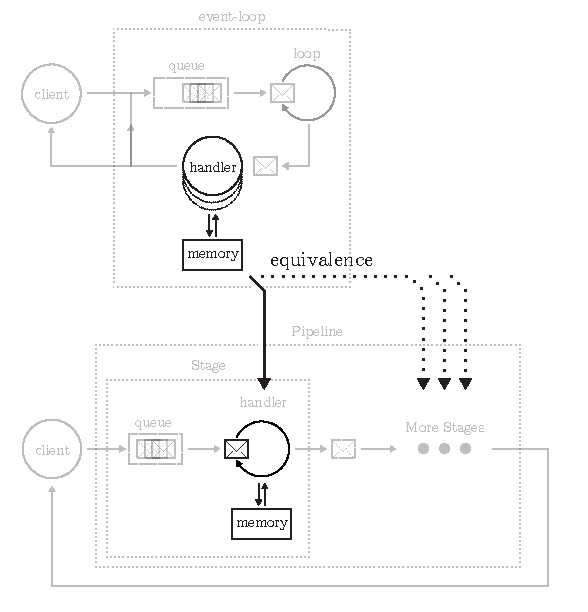
\includegraphics[width=0.8\linewidth]{../resources/equivalence.pdf}
  \label{fig:equivalence}
  \caption{equivalence}
\end{figure}

\subsection{Continuous Development}


This transformation allows developers to constantly keep two organizations of their implementation. %, allowing them to start with productivity, and seamlessly abandon it for efficiency as the project matures.
At first, developers start development with the productivity of the multi-paradigms languages, such as Javascript, following the global memory abstraction and the asynchronous control glow of the event-driven execution model.
The focus remains on productivity of development rather than the efficiency of execution.
The transformation of the application yields an execution at least as efficient as the original event-driven execution model.
Then, continuously during the maturation of the application, the focus shift towards efficiency.
The transformation of the application helps developers to enforce efficiency through continuous iteration to isolate stages.
They can identify, and arrange the implementation so as to remove the dependencies avoiding parallelism.

The next paragraphs present the event-driven execution model as the source of this transformation, and the pipeline architecture as the target.